%%%%%%%%%%%%%%%%%%%%%%%%%%%%%%%%%%%%%%%%%%%%%%%%%%%%%%%%%%%%%%%%%%%%%%%%%%%%%%%%
% ISE Lab -- Strips
% Giovanni Ciatto
% Alma Mater Studiorum - Università di Bologna
% mailto:giovanni.ciatto@unibo.it
%%%%%%%%%%%%%%%%%%%%%%%%%%%%%%%%%%%%%%%%%%%%%%%%%%%%%%%%%%%%%%%%%%%%%%%%%%%%%%%%
%\documentclass[handout]{beamer}\mode<handout>{\usetheme{default}}
%
\documentclass[presentation]{beamer}\mode<presentation>{\usetheme{AMSBolognaFC}}
%\documentclass[handout]{beamer}\mode<handout>{\usetheme{AMSBolognaFC}}
%%%%%%%%%%%%%%%%%%%%%%%%%%%%%%%%%%%%%%%%%%%%%%%%%%%%%%%%%%%%%%%%%%%%%%%%%%%%%%%%
\usepackage{ise-lab-common}
\usepackage{ise-lab-strips}
% version
\newcommand{\versionmajor}{1}
\newcommand{\versionminor}{0}
\newcommand{\versionpatch}{3}
\newcommand{\version}{\versionmajor.\versionminor.\versionpatch}
%%%%%%%%%%%%%%%%%%%%%%%%%%%%%%%%%%%%%%%%%%%%%%%%%%%%%%%%%%%%%%%%%%%%%%%%%%%%%%%%
\title[\currentLab{} -- STRIPS in Prolog]{Planning in STRIPS with Prolog}
%
\subtitle{\courseName{} / Module \moduleN{} (\courseAcronym)}
%
\author[\sspeaker{\gcShort}]{\speaker{\gcFull} \\ \gcEmail}
%
\institute[\disiShort, \uniboShort]{\disi{} (\disiShort)\\\unibo}
%
\date[A.Y. \academicYear{} (v.\ \version)]{Academic Year \academicYear{}\\(version \version)}
%
%%%%%%%%%%%%%%%%%%%%%%%%%%%%%%%%%%%%%%%%%%%%%%%%%%%%%%%%%%%%%%%%%%%%%%%%%%%%%%%%
\begin{document}
%%%%%%%%%%%%%%%%%%%%%%%%%%%%%%%%%%%%%%%%%%%%%%%%%%%%%%%%%%%%%%%%%%%%%%%%%%%%%%%%

%/////////
\frame{\titlepage}
%/////////

%%===============================================================================
\section*{Outline}
%%===============================================================================
%
%%/////////
\frame[c]{\tableofcontents[hideallsubsections]}
%%/////////

%===============================================================================
\section{Getting Started}
%===============================================================================

%/////////
\begin{frame}[c,allowframebreaks]{The Provided Project}

\begin{itemize}
    \item clone the provided source from the following Git repository
    %
    \begin{center}
        \uurl{https://dvcs.apice.unibo.it/pika-lab/courses/ise/ay2324/lab-3}
    \end{center}
    %
    \item inspect the project structure
    %
    \begin{figure}
        \centering
        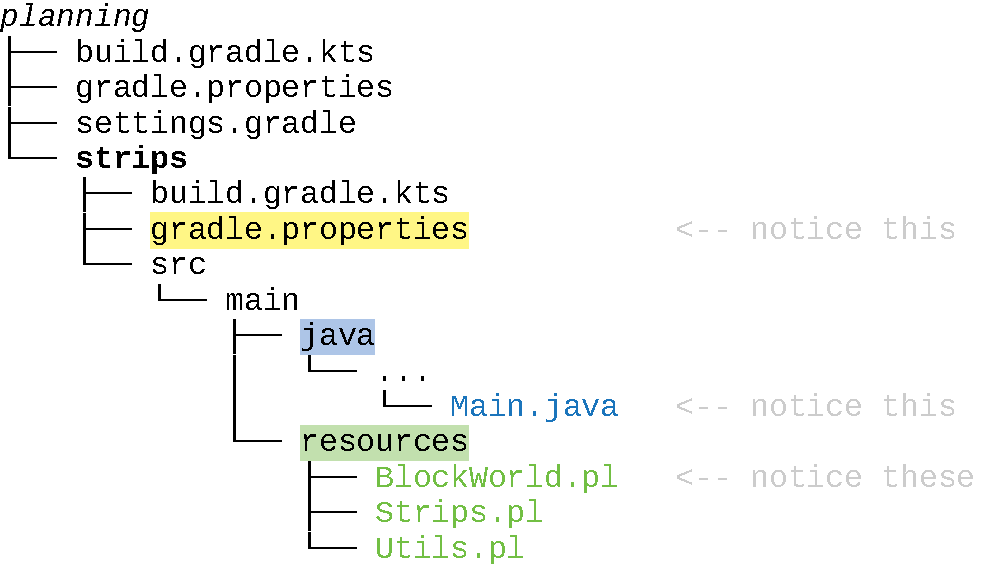
\includegraphics[width=.7\linewidth]{figures/treestructre.pdf}
    \end{figure}
\end{itemize}
%
\framebreak
%
Assuming a shell is open into the project's root directory, \texttt{planning/} \ldots
%
%
\begin{itemize}
    \item you can open a \tuprolog{} IDE, as usual, by running
    %
    \clicmd{./gradlew tuprologGui}
    %
    \item similarly, you can start the \tuprolog{} REPL by running
    %
    \clicmd{./gradlew tuprologRepl}
    %
    \item but most of the work will be done into the \alert{\texttt{strips/}} subproject and directory
\end{itemize}
\end{frame}
%/////////

%/////////
\begin{frame}{The \texttt{strips} Subproject}

The \texttt{strips/} subproject is composed by \ldots{}
%
\vfill
%
\begin{itemize}
    \item the \texttt{it.unibo.ise.lab.strips.\alert{Main}} Kotlin class
    %
    \begin{itemize}
        \item essentially implementing a simple REPL with some handy defaults
        \item you are not required to edit this
    \end{itemize}

    \vfill

    \item a folder of Prolog theories (i.e., \texttt{.pl} files), namely, \texttt{src/main/\alert{resources}}
    %
    \begin{itemize}
        \item you will be required to edit some of them
    \end{itemize}

    \vfill

    \item a \texttt{gradle\alert{.properties}} file, which will affect the way the \texttt{Main} program behaves
    %
    \begin{itemize}
        \item you may need to edit it, several times
    \end{itemize}
\end{itemize}
\end{frame}


%/////////
\begin{frame}{The \texttt{it.unibo.ise.lab.strips.\alert{Main}} REPL Behaviour}

\begin{itemize}
    \item upon start up, the aforementioned \texttt{Main} program loads both the \texttt{Strips.pl} and \texttt{Utils.pl} theories
    %
    \begin{description}
        \item[\texttt{Strips.pl}] is where you will put your STRIPS implementation, and the model-agnostic rules

        \item[\texttt{Utils.pl}] contains several utility rules; you must \alert{understand} them; you are \emph{not} supposed to alter them
    \end{description}

    \item if no \texttt{'\alert{goal}'} or \texttt{'\alert{initialState}'} entries are provided in  \texttt{gradle.properties}, the \texttt{Main} program acts as a regular REPL
    \vfill

    \item otherwise, it will attempt to exploit the strips algorithm -- implemented by you -- on the provided \texttt{\alert{initialState}}, trying to reach \texttt{\alert{goal}}

    \item in any case, if the \texttt{'\alert{world}'} entry is present, the \texttt{Main} program will load the corresponding \texttt{.pl} file too
    %
    \begin{itemize}
        \item[e.g.] the \texttt{BlockWorld.pl} file
    \end{itemize}
\end{itemize}

\end{frame}

%===============================================================================
\section{STRIPS Overview}
%===============================================================================

\begin{frame}[allowframebreaks]
\frametitle{Stanford Research Institute Problem Solver (STRIPS)}

\begin{itemize}
    \item STRIPS is the very first successful attempt of building a Planner
\end{itemize}

%\vfill

\begin{block}{Automatic planner \textit{(recall)}}
    An \alert{automatic planner} is an algorithm accepting as input
    \begin{itemize}
        \item[(i)] a representation of some \alert{initial state},
        \item[(ii)] a \emph{set} of possible \alert{actions},
        \item[(iii)] a \alert{goal}, that is, a compact description of a target state,
    \end{itemize}
    and producing a \alert{plan} as output, that is, a \emph{sequence} or \emph{directed graph} of actions leading the described system from the initial to the target state

\end{block}

\vfill

\begin{block}{STRIPS}
    \begin{itemize}
        \item[+] action, world, and goal \alert{representation languages}
        %
        \begin{itemize}
            \item simpler -- thus less expressive -- than the situation calculus
            \item no frame problem
        \end{itemize}
        %
        \item[+] \alert{regression} planning $\implies$ \alert{backward} algorithm for building plans
        %
        \begin{itemize}
            \item search occurs on the \alert{state space}
            \item backward $\approx$ starting from the goal, move towards the initial goal
        \end{itemize}
    \end{itemize}
\end{block}

\end{frame}

\begin{frame}[allowframebreaks]{STRIPS in a Nutshell}

In STRIPS \ldots

\begin{block}{How are \aalert{states} represented?}
    \begin{itemize}
        \item a state $S = \{ f_1, \ldots, f_n\}$ is a \alert{set} of \alert{fluents} $f_i$
        \item each fluent $f$ is a \emph{ground} logic \alert{fact} which is true in that state
        \item CWA: only what is \emph{explicitly} stated, is true
    \end{itemize}
\end{block}

\begin{block}{How are \aalert{goals} represented?}
    \begin{itemize}
        \item a goal $S = \{ f_1, \ldots, f_m\}$ is a \alert{(sub-)set} of \alert{fluents} $f_j$
        \item every fluent in the goal must be \alert{included} in a state, for the goal to hold in that state
        \begin{itemize}
            \item[i.e.] $G \text{ holds in } S \Leftrightarrow G \subseteq S$
        \end{itemize}
        \item[$\rightarrow$] Goal testing $\equiv$ Set inclusion
        \begin{itemize}
            \item[$\rightarrow$] no entailment notion $\rightarrow$ less computational effort, less expressivity
        \end{itemize}
    \end{itemize}
\end{block}

\framebreak

\begin{block}{How are \aalert{actions} represented?}
    An action $\alpha$ is a quartet $\langle N, P, A, D \rangle$, where
    \begin{itemize}
        \item[$N$] is the action name
        \item[$P$] is a set of fluents, representing \alert{pre}-conditions
        \item[$A$] is a set of fluents, representing \alert{positive post}-conditions
        \begin{itemize}
            \item a.k.a.\ $A$dd List
        \end{itemize}
        \item[$D$] is a set of fluents, representing \alert{negative post}-conditions
        \begin{itemize}
            \item a.k.a. $D$elete List, or Remove List
        \end{itemize}
    \end{itemize}
\end{block}

\begin{alertblock}{STRIPS assumption}
    What is \textbf{not} specified in $A$ or $D$ remains unchanged
    \begin{itemize}
        \item[$\rightarrow$] no frame problem!
    \end{itemize}
\end{alertblock}

\begin{block}{First-order logic (FOL)}
    Fluents and action names in STRIPS are FOL \alert{terms}, subject to the following constraints:
    %
    \begin{itemize}
        \item states can only contain \alert{ground} terms
        \item gaols and action names may contain \alert{variables}
        \item variables contained in an action name $N$ can occur in fluents from $P$, $A$, or $D$ too
    \end{itemize}
\end{block}

\framebreak

\begin{block}{Action applicability}
    An action $\alpha = \langle N, P, A, D \rangle$ is \alert{applicable} to some state $S$ if and only if there exists some $S' \subseteq S$ such that:
    %
    \begin{center}
        $mgu(S', P) = \theta$
    \end{center}
    %
%	where $mgu$ is the \emph{most general unifier} function, returning a substitution $\theta$ which can make $P$ equals to $S'$ when applied to $P$.
    %
    which implies $P / \theta \subseteq S$.
\end{block}
%
\begin{itemize}
    %
    \item there, $mgu$ is the \emph{most general unifier} function, returning a substitution $\theta$ which can make $P$ equals to $S'$ when applied to $P$.
    %
    \item roughly speaking, $mgu(S', P) = \theta$ can be read as ``$P$ unifies with $S'$''
    %
\end{itemize}

\begin{block}{Action application}
    Assuming some action $\alpha = \langle N, P, A, D \rangle$ is applicable to some state $S_1$ through $\theta$, it can be applied to $S_1$ by means of the following function:
    \begin{center}
         $apply(S_1, \alpha) = S_2 = \alert{(S_1 - D / \theta) \cup A / \theta} $
    \end{center}
    which, essentially, formally describes the STRIPS assumption
\end{block}

\end{frame}

\section{The STRIPS Planner in Prolog (I)}

\subsection{States}

\begin{frame}[allowframebreaks]{Modelling STRIPS States in Prolog}

Using your Prolog IDE, or some pencil \& paper (i.e., nothing to run here)

\startExercise

\begin{block}{Exercise \currentExercise{}a -- The Block World}
       Design the states of a world made of \emph{named} \alert{blocks}.
       Blocks may either be on the \alert{table}, or stack'd up\alert{on} each others.
       Their top faces may thus \alert{clear} or occupied by another block.
       A robotic \emph{hand} is part of the world.
       It may be either \alert{holding} a block or \alert{free}.
\end{block}

\begin{block}{Exercise \currentExercise{}b -- The Register Machine}
    Design the states of a \emph{register machine} made up of a number of \emph{named} \alert{registers}, each one storing an integer value.
\end{block}

\framebreak

\begin{block}{Exercise \currentExercise{}c -- Alice and Bob's City}
    \begin{columns}
        \begin{column}{.7\linewidth}
            Consider the Alice's city topology shown on the right, where vertices represent places, and edges represent roads.
            Alice and her son Bob live at \alert{\texttt{h}}ome.
            Bob's \alert{\texttt{s}}chool is close to \alert{\texttt{h}}ome, but needs to step through the super\alert{\texttt{m}}arket to go to \alert{\texttt{w}}ork.
            They own a car.
            Both Alice and Bob can either be in any of the four mentioned places, or on the car.
            The car too can be in any of the four mentioned places.
            It can contain 0, 1, or 2 people.
        \end{column}
        \begin{column}{.3\linewidth}
            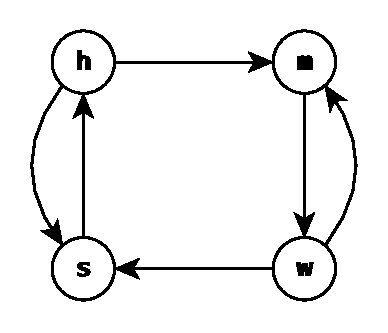
\includegraphics[width=\linewidth]{./figures/city.pdf}
        \end{column}
    \end{columns}
\end{block}

\begin{itemize}
    \item try thinking about \alert{how} (i.e. which Prolog syntax) you would use to model such situations

    \item once you are done, rise your hand and ask for feedbacks
\end{itemize}
\end{frame}

\begin{frame}[allowframebreaks]{Example: Modelling states for the Block World}

One possible solution
%
\begin{itemize}
    \item blocks are identified by constants, e.g. \prolog{a}, \prolog{b}, \prolog{c}, etc
    \vfill
    \item a fluent in the form \prolog{ontable(X)} states that the block referenced by \prolog{X} lays on the table
    \vfill
    \item a fluent in the form \prolog{on(X, Y)} states that the block referenced by \prolog{X} lays on top of the block referenced by \prolog{Y}
    \vfill
    \item a fluent in the form \prolog{clear(X)} states that the top face of the block referenced by \prolog{X} is clear
    \vfill
    \item a fluent in the form \prolog{holding(X)} states that the robotic hand is holding the block referenced by \prolog{X}
    \vfill
    \item the fluent \prolog{handempty} states that the robotic hand is free
\end{itemize}

\framebreak

Consider for instance state $S =\ $\prolog{[on(a,c),ontable(b),ontable(c),clear(a),clear(b),holding(d)]}\footnote{Sets in Prolog are represented as lists!}
%
\begin{center}
\lstinputlisting[xleftmargin=.40\linewidth, xrightmargin=.20\linewidth]{./listings/block0.txt}
\end{center}

\end{frame}

\subsection{Actions}

\begin{frame}[c]{STRIPS Actions in Prolog}

\begin{block}{Conventions}
    In this lab we represent actions as Prolog facts matching the following structure
    %
    \begin{center}
        \prolog{action(N, if(P), '+'(A), '-'(D)).}
    \end{center}
    where \prolog{N} is a structure, and \prolog{P}, \prolog{A}, and \prolog{D} are lists of fluents

\end{block}

\begin{exampleblock}{Consider for instance \texttt{BlockWorld.pl}}
    \lstinputlisting[frame=none,xleftmargin=.20\linewidth, xrightmargin=.20\linewidth,style=Prolog-cool,basicstyle=\scriptsize\ttfamily]{./listings/BlockWorld.txt}
\end{exampleblock}

\end{frame}

\begin{frame}[allowframebreaks]{Modelling STRIPS Actions in Prolog}

Using your Prolog IDE, or some pencil \& paper (i.e., nothing to run here)
%
\begin{itemize}
    \item save each exercise in a different \texttt{.pl} file in \texttt{src/main/\alert{resources}}
\end{itemize}

\begin{block}{Exercise 1a -- Actions for the Block World (\texttt{BlockWorld.pl})}
       \begin{description}
           \item[\texttt{stack}] --- if a block's top face is clear, and the robotic hand is holding another block, this action let the hand put the letter block on top of the former

           \item[\texttt{unstack}] --- if a block's top face is clear, and it is laying on top of another block, and the robotic hand is free, this action let the hand grab the former block

           \item[\texttt{pick}] --- if a block's top face is clear, and it is laying on the table, and the robotic hand is free, this action let the hand grab that block

           \item[\texttt{put}] --- if the robotic hand is holding a block, this action let the hand put such block on the table
       \end{description}
\end{block}

\begin{block}{Exercise 1b -- Actions for the Register Machine (\texttt{Registers.pl})}
       \begin{description}
           \item[\texttt{inc}] --- increases a register by one, given the register name
           \item[\texttt{dec}] --- decreases a register by one, given the register name
           \item[\texttt{sum}] --- sums up the values of two registers, given their names, and stores the resulting value into a third register, given its name
           \item[\texttt{sub}] --- like \texttt{sum}, but subtracting
       \end{description}
\end{block}

\begin{block}{Exercise 1c -- Actions for Alice's City (\texttt{City.pl})}
       \begin{description}
           \item[\texttt{getin}] --- let either Alice or Bob enter the car, if he / she is not yet in the car, and he / she is in the same place the car currently is
           \item[\texttt{getout}] --- let either Alice or Bob exit the car in the place where the car currently is, assuming he / she is already in the car
           \item[\texttt{driveto}] --- moves the car from its current position to some destination, assuming that Alice is in the car -- since Bob has no driving license -- and that the destination is reachable from the car's current position
       \end{description}
\end{block}

\begin{itemize}
    \item try thinking about \alert{how} (i.e. which Prolog syntax) you would use to model such actions

    \item once you are done, rise your hand and ask for feedbacks
\end{itemize}
\end{frame}


\subsection{Actions Application}

\begin{frame}[c]{Actions Application}

    \begin{itemize}
        \item the action application function $apply(\cdot, \cdot)$ can be implemented in Prolog by means of a ternary relation with the following signature:
        %
        \begin{center}
            \prolog{apply(+State, +ActionName, -NewState)}
        \end{center}
        %
        which succeeds in computing the novel state \prolog{NewState} only if the action named \prolog{ActionName} is applicable to \prolog{State}

        \vfill

        \item its implementation relies on the set operations contained in \texttt{Utils.pl}

%		\vfill
%
%		\item \ldots{} and on a number of accessor relations contained in \texttt{Strips.pl}

        \vfill

        \item \ldots{} other than, of course, Prolog's builtins such as \texttt{member/2}
    \end{itemize}
\end{frame}

\begin{frame}[c]{The \texttt{Utils.pl} Library}

    The \texttt{Utils.pl} library exposes a number of useful Prolog rules which must \textbf{not} be implemented:
    %
    \vfill
    %
    \begin{itemize}
        \item set comparisons %(general signature: \prolog{<rule name>(+Set1, +Set2)})
        %
        \begin{itemize}
            \item \prolog{subset(+S1,+S2)}, \prolog{subseteq(+S1,+S2)}, \prolog{eq(+S1,+S2)}, \prolog{neq(+S1,+S2)}, \prolog{superset(+S1,+S2)}, \prolog{superseteq(+S1,+S2)}
            \item implementing $S_1 \subset S_2$, $S_1 \subseteq S_2$, $S_1 \equiv S_2$, $S_1 \not\equiv S_2$, $S_1 \supset S_2$, $S_1 \supseteq S_2$, respectively
        \end{itemize}

        \vfill

        \item set operations
        %
        \begin{itemize}
            \item \prolog{union(+S1,+S2,-S3)} implementing $S3 = S1 \cup S2$
            \item \prolog{intersection(+S1,+S2,-S3)} implementing $S3 = S1 \cap S2$
            \item \prolog{difference(+S1,+S2,-S3)} implementing $S3 = S1 - (S1 \cup S2)$
        \end{itemize}

        \vfill

        \item membership
        %
        %
        \begin{itemize}
            \item \prolog{member(?X,+S)} implementing $X \in S$ \hfill {\small (this is actually standard Prolog)}
            \item \prolog{in(?X,+S)} alias for \texttt{member/2}
        \end{itemize}
    \end{itemize}
\end{frame}

%\begin{frame}[c]{The Provided Rules in \texttt{Strips.pl}}
%
%	The \texttt{Strips.pl} library comes with a number of already implemented rules, such as:
%	%
%	\begin{itemize}
%		\item accessors for preconditions:
%		%
%		\begin{itemize}
%			\item \prolog{preconditions(+ActionName, -PreconditionList)} retrieves all the pre-conditions of an action, given its name
%			\item \prolog{precondition(+ActionName, -Precondition)} selects one pre-condition from an action, given its name
%		\end{itemize}
%
%		\item accessors for positive post-conditions:
%		%
%		\begin{itemize}
%			\item \prolog{positive_effects(+ActionName, -AddList)} retrieves all the positive post-conditions of an action, given its name
%			\item \prolog{positive_effect(+ActionName, -Effect)} selects one positive post-condition from an action, given its name
%		\end{itemize}
%
%		\item accessors for negative post-conditions:
%		%
%		\begin{itemize}
%			\item \prolog{negative_effects(+ActionName, -DeleteList)} retrieves all the negative post-conditions of an action, given its name
%			\item \prolog{negative_effect(+ActionName, -Effect)} selects one negative post-condition from an action, given its name
%		\end{itemize}
%	\end{itemize}
%\end{frame}

\begin{frame}[c]{Implementing the \texttt{apply/3} relation}
    \begin{block}{Exercise 2 -- The \texttt{apply/3} relation}
        Fill the \texttt{apply/3} relation's code in \texttt{Strips.pl}, in such a way that it correctly implements the $apply(\cdot, \cdot)$ function
    \end{block}

    \begin{exampleblock}{Test if it behaves consistently with your actions}
        \footnotesize
        For instance, according to our modelling of the Block World:
        %
        \begin{itemize}
            \item \plil{apply([ontable(a), clear(a), handempty], pick(a), S)}
            %
            \begin{itemize}
                \item produces \plil{S / [holding(a)]}
            \end{itemize}

            \item \plil{apply([ontable(a), clear(a), handempty], put(a), S)} fails

            \item \plil{apply([ontable(a),clear(b),on(b,a),handempty],unstack(b,X),S)}
            %
            \begin{itemize}
                \item produces \plil{S / [ontable(a), clear(a), holding(a)]}
            \end{itemize}

            \item \plil{apply([ontable(a),clear(b),on(b, a),handempty],stack(b,X),S)}
            %
            \begin{itemize}
                \item fails
            \end{itemize}
        \end{itemize}
    \end{exampleblock}
\end{frame}

\begin{frame}[c]{Testing Your Code}

    \begin{itemize}
        \item you can test your \texttt{apply/3} implementation against the actions you defined, say, into \texttt{BlockWorld.pl}, by uncommenting the line
        %
        \clicmd{world=\alert{BlockWorld}}
        %
        within \texttt{gradle.properties} file

        \vfill

        \item then, you can start a Prolog REPL by running
        %
        \clicmd{./gradlew :strips:run}
        %
        and then provide your \emph{dot-terminated} queries through \texttt{stdin}

        \vfill

        \item similarly, you can test other action files by changing the value of the \texttt{world} property in \texttt{gradle.properties}

        \vfill

        \item remember to restart your REPL if you edit any \texttt{.pl} file
    \end{itemize}

\end{frame}


\section{The STRIPS Algorithm}

\subsection{Formal Description}

\begin{frame}[c]{The STRIPS Algorithm -- Required Definitions}

Let
%
\begin{itemize}
    \item $[ Head \mid Tail ]$ denote a stack whose head is $Head$ and where other elements are represented by $Tail$

    \vfill

    \item $Actions$ be a set of action names, ranged by $N$

    \vfill

    \item $State$, $State_0$ be states, i.e. sets of fluents, ranged by $F$

    \vfill

    \item $pre(N) \mapsto G_1 \wedge \ldots \wedge G_n$ the function mapping each action name $N$ to the conjunction of preconditions of $N$

    \vfill

    \item $post_+(N) \mapsto \{G_1, \ldots, G_n\}$ the function mapping each action name $N$ to the set of positive effects of $N$

    \vfill

    \item $apply(State, N) \mapsto State'$ be the function mapping a state-action-name couple to the state attained by applying that action to that state
\end{itemize}

\end{frame}

\begin{frame}[c]{The STRIPS Algorithm -- Pseudo-code \hfill {\scriptsize(CP = Choice Point)}}

% 	\begin{block}{Pseudocode \hfill CP = Choice Point}
        \begin{algorithmic}\small
            \Function{Strips}{$State_0$, $Actions$, $Goal \equiv G_1 \wedge \dots \wedge G_n$}

                \State $State \leftarrow State_0$; ~ $Stack \leftarrow [G_1 \wedge \dots \wedge G_n]$; ~ $Plan \leftarrow []$

                \State

                \While{$Stack \equiv [\alert{H} \mid Tail]$} \Comment{while $Stack$ is not empty}
                    % \State $X \leftarrow head(Stack)$
                    \If{$\exists F \in State : mgu(\alert{H}, F) = \theta$}
                        \State $Stack \leftarrow Tail / \theta$ \Comment{Pop}
                    \ElsIf{$\exists N \in Actions : \exists E \in post_{+}(N) : mgu(\alert{H}, E) = \theta$} \Comment{\alert{CP}}
                        %\State $Stack \leftarrow tail(Stack)\theta$
                        \State $Stack \leftarrow [pre(N), N \mid Tail] / \theta$  \Comment{Pop; Push($N$); Push($pre(N)$)}
                    \ElsIf{$\alert{H} \equiv G_1 \wedge \ldots \wedge G_m$}
                        \State $Stack \leftarrow [G_1, \ldots, G_m \mid Tail]$ \Comment Pop, Push($G_1$), \ldots, Push($G_m$), \alert{CP}
                    \ElsIf{$\alert{H} \in Actions$}
                        \State $State \leftarrow apply(State, H)$
                        \State $Plan \leftarrow [H \mid Plan]$
                    \Else
                        \State \Return $\varnothing$ \Comment Failure
                    \EndIf
                \EndWhile

                \State

                \State \Return reverse($Plan$) \Comment Success
            \EndFunction
        \end{algorithmic}
% 	\end{block}

\end{frame}

\begin{frame}[c,allowframebreaks]{The STRIPS Algorithm -- Remarks}
%
 \begin{itemize}
     \item it accepts as input ($\rightarrow$), and produces as output ($\leftarrow$)
    %
    \begin{itemize}
        \item[$\rightarrow$] the initial state $State_0$ (i.e. a set of fluents)
        \item[$\rightarrow$] a set of action \alert{names} $Actions$
        \item[$\rightarrow$] the goal to be reached, $Goal$, i.e. a \alert{conjunction} of fluents
        \item[$\leftarrow$] either a plan (i.e., a \alert{sequence} of action names) or $\varnothing$, in case none exists
    \end{itemize}
    %
    \item it leverages on three data structures
    %
    \begin{itemize}
        \item[State] which represents the currently simulated state (initialised to $State_0$)
        \item[Stack] which \emph{orderly} stores the currently \emph{unsatisfied} goals and \emph{unapplied} actions (initialised as the singleton list storing $Goal$)
        \item[Plan] which stores the actions names of the actions simulated so far, in such a way that its reverse is always a (partial) plan (initialised as the empty list)
    \end{itemize}
\end{itemize}
%
\framebreak
%
\begin{itemize}
    \item it leverages on the following functions, apart from $mgu(\cdot,\cdot)$
    %
    \begin{description}\small
        \item[$pre(N)$] given an action name $N$, it returns the set of pre-conditions of the corresponding action, as a \alert{conjunction} of fluents
        \item[$post_{+}(N)$] given an action name $N$, it returns the set of \alert{positive} post-conditions of the corresponding action, as a \alert{set} of fluents
        \item[$apply(S, N)$] given a state $S$ and an action name $N$, it returns the state achieved by applying the corresponding action in $S$
        \item[$reverse(L)$] it reverses the list $L$ provided as input
    \end{description}
    %
    \item it is characterised by the following \alert{choice points}
    %
    \begin{itemize}
        \item how the next action to be applied is selected, in case more than one are applicable
        \item how (i.e. in which order) unsatisfied sub-goals are selected for searching a sub-plan satisfying them
    \end{itemize}
    %
    \item[!!] the particular choices performed at \alert{each} choice point may heavily affect the effectiveness and performance of STRIPS
\end{itemize}
\end{frame}

\begin{frame}%[shrink]
\small
\frametitle{The STRIPS Algorithm -- Explanation}

    Repeat until $Stack$ is empty. Let $H$ the head of the $Stack$:
    %
    % At each step, the action performed by the algorithm depends on the stack's head, $H$:
    %
    \begin{enumerate}
        \item if $H$ unifies through $\theta$ with some fluent $F$ in the current $State$:
        %
        \begin{itemize}
            \item then $H$ is popped and $\theta$ is applied to $Stack$'s tail
        \end{itemize}

        \vfill

        \item if $H$ matches some \alert{positive} post-condition $A$ of some action named $N$:
        %
        \begin{itemize}
            \item then $H$ is popped, $N$ is pushed, as well as $pre(N)$
            \item and $\theta = mgu(H, A)$ is applied to $Stack$
        \end{itemize}

        \vfill

        \item if $H$ matches some conjunction of goals $G_1 \wedge \ldots \wedge G_m$:
        %
        \begin{itemize}
            \item then the conjuction is popped
            \item and each $G_i$, for $i \in \{1,\ldots,m\}$ is pushed on the stack
            \item the ordering of such pushings is arbitrary
        \end{itemize}

        \vfill

        \item if $H$ matches some action name:
        %
        \begin{itemize}
            \item then $H$ is applied to $State$ and $State$ is updated accordingly
            \item furthermore, $H$ is pushed into $Plan$
        \end{itemize}

        \vfill

        \item otherwise, no plan can be computed and $\varnothing$ is returned
    \end{enumerate}

    \vfill

    When $Stack$ is empty, $reverse(Plan)$ is returned

\end{frame}

\subsection{Example}

\newcounter{StripsExampleStep}
\newcommand{\nextStripsExampleStep}{\stepcounter{StripsExampleStep}\theStripsExampleStep}

\begin{frame}[c]{The STRIPS Algorithm -- Example}
    \small

    \begin{exampleblock}{Step \theStripsExampleStep \hfill $Plan = []$}
        \begin{columns}[t]
            \begin{column}{.30\linewidth}\centering
                State

                \texttt{[clear(b), clear(c), on(c,a), ontable(a), ontable(b), handempty]}
            \end{column}
            \begin{column}{.50\linewidth}\centering
                Stack
                %
                \begin{itemize}
                    \item \texttt{on(a,c) $\wedge$ on(c,b)}
                \end{itemize}
            \end{column}
            \begin{column}{.10\linewidth}\centering
                Example

                \lstinputlisting{./listings/strips-example.0.txt}
            \end{column}
        \end{columns}
    \end{exampleblock}

\end{frame}

\begin{frame}[c]{The STRIPS Algorithm -- Example}
\small

    \begin{exampleblock}{Step \nextStripsExampleStep{} \hfill $Plan = []$}
        \begin{columns}[t]
            \begin{column}{.30\linewidth}\centering
                \texttt{[clear(b), clear(c), on(c,a), ontable(a), ontable(b), handempty]}
            \end{column}
            \begin{column}{.50\linewidth}\centering
                \begin{itemize}
                    \item \texttt{on(c,b)}
                    \item \texttt{on(a,c)}
                % 	\item \texttt{on(a,c) $\wedge$ on(c,b)}
                \end{itemize}
            \end{column}
            \begin{column}{.10\linewidth}\centering
                \lstinputlisting{./listings/strips-example.0.txt}
            \end{column}
        \end{columns}
    \end{exampleblock}

\end{frame}

\begin{frame}[c]{The STRIPS Algorithm -- Example}
\small

    \begin{exampleblock}{Step \nextStripsExampleStep{} \hfill $Plan = []$}
        \begin{columns}[t]
            \begin{column}{.30\linewidth}\centering
                \texttt{[clear(b), clear(c), on(c,a), ontable(a), ontable(b), handempty]}
            \end{column}
            \begin{column}{.50\linewidth}\centering
                \begin{itemize}
                    \item \texttt{clear(b) $\wedge$ holding(c)}
                    \item[!] \texttt{stack(c,b)}
                    \item \texttt{on(a,c)}
                % 	\item \texttt{on(a,c) $\wedge$ on(c,b)}
                \end{itemize}
            \end{column}
            \begin{column}{.10\linewidth}\centering
                \lstinputlisting{./listings/strips-example.0.txt}
            \end{column}
        \end{columns}
    \end{exampleblock}

    \vfill

    \footnotesize
    Notice
    \begin{itemize}\tiny
        \item selected action \texttt{stack(c, b)} to satisfy goal \texttt{on(c,b)}
    \end{itemize}

\end{frame}

\begin{frame}[c]{The STRIPS Algorithm -- Example}
\small

    \begin{exampleblock}{Step \nextStripsExampleStep{} \hfill $Plan = []$}
        \begin{columns}[t]
            \begin{column}{.30\linewidth}\centering
                \texttt{[clear(b), clear(c), on(c,a), ontable(a), ontable(b), handempty]}
            \end{column}
            \begin{column}{.50\linewidth}\centering
                \begin{itemize}
                    \item \texttt{holding(c)}
                    \item \texttt{clear(b)}
                % 	\item \texttt{clear(b) $\wedge$ holding(c)}
                    \item[!] \texttt{stack(c,b)}
                    \item \texttt{on(a,c)}
                % 	\item \texttt{on(a,c) $\wedge$ on(c,b)}
                \end{itemize}
            \end{column}
            \begin{column}{.10\linewidth}\centering
                \lstinputlisting{./listings/strips-example.0.txt}
            \end{column}
        \end{columns}
    \end{exampleblock}

\end{frame}

\begin{frame}[c]{The STRIPS Algorithm -- Example}
\small

    \begin{exampleblock}{Step \nextStripsExampleStep{} \hfill $Plan = []$}
        \begin{columns}[t]
            \begin{column}{.30\linewidth}\centering
                \texttt{[clear(b), clear(c), on(c,a), ontable(a), ontable(b), handempty]}
            \end{column}
            \begin{column}{.50\linewidth}\centering
                \begin{itemize}
                    \item \texttt{clear(c) $\wedge$ handempty $\wedge$ on(c, Y)}
                    \item[!] \texttt{unstack(c, Y)}
                    \item \texttt{clear(b)}
                % 	\item \texttt{clear(b) $\wedge$ holding(c)}
                    \item[!] \texttt{stack(c,b)}
                    \item \texttt{on(a,c)}
                % 	\item \texttt{on(a,c) $\wedge$ on(c,b)}
                \end{itemize}
            \end{column}
            \begin{column}{.10\linewidth}\centering
                \lstinputlisting{./listings/strips-example.0.txt}
            \end{column}
        \end{columns}
    \end{exampleblock}

    \vfill

    \footnotesize
    Notice
    \begin{itemize}\tiny
        \item selected action \texttt{unstack(c, Y)} to satisfy goal \texttt{holding(c)}
    \end{itemize}

\end{frame}

\begin{frame}[c]{The STRIPS Algorithm -- Example}
\small

    \begin{exampleblock}{Step \nextStripsExampleStep{} \hfill $Plan = []$}
        \begin{columns}[t]
            \begin{column}{.30\linewidth}\centering
                \texttt{[clear(b), \alert{clear(c)}, on(c,a), ontable(a), ontable(b), handempty]}
            \end{column}
            \begin{column}{.50\linewidth}\centering
                \begin{itemize}
                    \item \alert{\texttt{clear(c)}}
                    \item \texttt{on(c, Y)}
                    \item \texttt{handempty}
                % 	\item \texttt{clear(c) $\wedge$ handempty $\wedge$ on(c, Y)}
                    \item[!] \texttt{unstack(c, Y)}
                    \item \texttt{clear(b)}
                % 	\item \texttt{clear(b) $\wedge$ holding(c)}
                    \item[!] \texttt{stack(c,b)}
                    \item \texttt{on(a,c)}
                % 	\item \texttt{on(a,c) $\wedge$ on(c,b)}
                \end{itemize}
            \end{column}
            \begin{column}{.10\linewidth}\centering
                \lstinputlisting{./listings/strips-example.0.txt}
            \end{column}
        \end{columns}
    \end{exampleblock}

\end{frame}

\begin{frame}[c]{The STRIPS Algorithm -- Example}
\small

    \begin{exampleblock}{Step \nextStripsExampleStep{} \hfill $Plan = []$}
        \begin{columns}[t]
            \begin{column}{.30\linewidth}\centering
                \texttt{[clear(b), clear(c), \alert{on(c,a)}, ontable(a), ontable(b), handempty]}
            \end{column}
            \begin{column}{.50\linewidth}\centering
                \begin{itemize}
                    \item \alert{\texttt{on(c, Y)}}
                    \item \texttt{handempty}
                % 	\item \texttt{clear(c) $\wedge$ handempty $\wedge$ on(c, Y)}
                    \item[!] \texttt{unstack(c, Y)}
                    \item \texttt{clear(b)}
                % 	\item \texttt{clear(b) $\wedge$ holding(c)}
                    \item[!] \texttt{stack(c,b)}
                    \item \texttt{on(a,c)}
                % 	\item \texttt{on(a,c) $\wedge$ on(c,b)}
                \end{itemize}
            \end{column}
            \begin{column}{.10\linewidth}\centering
                \lstinputlisting{./listings/strips-example.0.txt}
            \end{column}
        \end{columns}
    \end{exampleblock}

    \vfill

    \footnotesize
    Notice
    \begin{itemize}\tiny
        \item goal \texttt{on(c, a)} can be satisfied if substitution \texttt{\{Y = a\}} is applied to the whole $Stack$
    \end{itemize}

\end{frame}

\begin{frame}[c]{The STRIPS Algorithm -- Example}
\small

    \begin{exampleblock}{Step \nextStripsExampleStep{} -- \texttt{Y/a} \hfill $Plan = []$}
        \begin{columns}[t]
            \begin{column}{.30\linewidth}\centering
                \texttt{[clear(b), clear(c), on(c,a), ontable(a), ontable(b), \alert{handempty}]}
            \end{column}
            \begin{column}{.50\linewidth}\centering
                \begin{itemize}
                    \item \alert{\texttt{handempty}}
                % 	\item \texttt{clear(c) $\wedge$ handempty $\wedge$ on(c, a)}
                    \item[!] \texttt{unstack(c, a)}
                    \item \texttt{clear(b)}
                % 	\item \texttt{clear(b) $\wedge$ holding(c)}
                    \item[!] \texttt{stack(c,b)}
                    \item \texttt{on(a,c)}
                % 	\item \texttt{on(a,c) $\wedge$ on(c,b)}
                \end{itemize}
            \end{column}
            \begin{column}{.10\linewidth}\centering
                \lstinputlisting{./listings/strips-example.0.txt}
            \end{column}
        \end{columns}
    \end{exampleblock}

\end{frame}

\begin{frame}[c]{The STRIPS Algorithm -- Example}
\small

    \begin{exampleblock}{Step \nextStripsExampleStep{}  -- Apply! \hfill $Plan = []$}
        \begin{columns}[t]
            \begin{column}{.30\linewidth}\centering
                \texttt{[clear(b), clear(c), on(c,a), ontable(a), ontable(b), handempty]}
            \end{column}
            \begin{column}{.50\linewidth}\centering
                \begin{itemize}
                % 	\item \texttt{clear(c) $\wedge$ handempty $\wedge$ on(c, a)}
                    \item[!] \texttt{unstack(c, a)}
                    \item \texttt{clear(b)}
                % 	\item \texttt{clear(b) $\wedge$ holding(c)}
                    \item[!] \texttt{stack(c,b)}
                    \item \texttt{on(a,c)}
                % 	\item \texttt{on(a,c) $\wedge$ on(c,b)}
                \end{itemize}
            \end{column}
            \begin{column}{.10\linewidth}\centering
                \lstinputlisting{./listings/strips-example.0.txt}
            \end{column}
        \end{columns}
    \end{exampleblock}

\end{frame}

% \begin{frame}%[allowframebreaks]
% \frametitle{The STRIPS algorithm -- Example}
% \small

% 	\begin{exampleblock}{Step \nextStripsExampleStep{} -- Apply! \hfill $Plan = []$}
% 		\begin{columns}[t]
% 			\begin{column}{.30\linewidth}\centering
% 				\texttt{[clear(b), clear(c), on(c,a), ontable(a), ontable(b), handempty]}
% 			\end{column}
% 			\begin{column}{.50\linewidth}\centering
% 				\begin{itemize}
% 					\item[!] \texttt{unstack(c, a)}
% 					\item \texttt{clear(b)}
% 				% 	\item \texttt{clear(b) $\wedge$ holding(c)}
% 					\item[!] \texttt{stack(c,b)}
% 					\item \texttt{on(a,c)}
% 				% 	\item \texttt{on(a,c) $\wedge$ on(c,b)}
% 				\end{itemize}
% 			\end{column}
% 			\begin{column}{.10\linewidth}\centering
% 				\lstinputlisting{./listings/strips-example.0.txt}
% 			\end{column}
% 		\end{columns}
% 	\end{exampleblock}

% \end{frame}

\begin{frame}[c]{The STRIPS Algorithm -- Example}
\small

    \begin{exampleblock}{Step \nextStripsExampleStep{} \hfill $Plan = [\mathtt{unstack(c,a)}]$}
        \begin{columns}[t]
            \begin{column}{.30\linewidth}\centering
                \alert{\texttt{[\emph{clear(b)}, clear(a), ontable(a), ontable(b), holding(c)]}}
            \end{column}
            \begin{column}{.50\linewidth}\centering
                \begin{itemize}
                    \item \alert{\emph{\texttt{clear(b)}}}
                % 	\item \texttt{clear(b) $\wedge$ holding(c)}
                    \item[!] \texttt{stack(c,b)}
                    \item \texttt{on(a,c)}
                % 	\item \texttt{on(a,c) $\wedge$ on(c,b)}
                \end{itemize}
            \end{column}
            \begin{column}{.10\linewidth}\centering
                \lstinputlisting{./listings/strips-example.1.txt}
            \end{column}
        \end{columns}
    \end{exampleblock}

\end{frame}

\begin{frame}[c]{The STRIPS Algorithm -- Example}
\small

\begin{exampleblock}{Step \nextStripsExampleStep{} -- Apply! \hfill $Plan = [\mathtt{unstack(c,a)}]$}
    \begin{columns}[t]
        \begin{column}{.30\linewidth}\centering
            \texttt{[clear(b), clear(a), ontable(a), ontable(b), holding(c)]}
        \end{column}
        \begin{column}{.50\linewidth}\centering
            \begin{itemize}
                % \item \texttt{clear(b) $\wedge$ holding(c)}
                \item[!] \texttt{stack(c,b)}
                \item \texttt{on(a,c)}
                % \item \texttt{on(a,c) $\wedge$ on(c,b)}
            \end{itemize}
        \end{column}
        \begin{column}{.10\linewidth}\centering
            \lstinputlisting{./listings/strips-example.1.txt}
        \end{column}
    \end{columns}
\end{exampleblock}

\end{frame}


% \begin{frame}[c]{The STRIPS Algorithm -- Example}
% \small

% \begin{exampleblock}{Step \nextStripsExampleStep{} \hfill $Plan = [\mathtt{unstack(c,a)}]$}
%     \begin{columns}[t]
%         \begin{column}{.30\linewidth}\centering
%             \alert{\texttt{[clear(b), clear(a), ontable(a), ontable(b), holding(c)]}}
%         \end{column}
%         \begin{column}{.50\linewidth}\centering
%             \begin{itemize}
%                 \item \texttt{on(a,c)}
%                 % \item \texttt{on(a,c) $\wedge$ on(c,b)}
%             \end{itemize}
%         \end{column}
%         \begin{column}{.10\linewidth}\centering
%             \lstinputlisting{./listings/strips-example.1.txt}
%         \end{column}
%     \end{columns}
% \end{exampleblock}

% \end{frame}


\begin{frame}%[allowframebreaks]
\frametitle{The STRIPS Algorithm -- Example}
\small

\begin{exampleblock}{Step \nextStripsExampleStep{} \hfill $Plan = [\mathtt{stack(c,b),unstack(c,a)}]$}
    \begin{columns}[t]
        \begin{column}{.30\linewidth}\centering
            \alert{\texttt{[on(c, b), clear(c), clear(a), ontable(a), ontable(b), handempty]}}
        \end{column}
        \begin{column}{.50\linewidth}\centering
            \begin{itemize}
                \item \texttt{on(a,c)}
                % \item \texttt{on(a,c) $\wedge$ on(c,b)}
            \end{itemize}
        \end{column}
        \begin{column}{.10\linewidth}\centering
            \lstinputlisting{./listings/strips-example.2.txt}
        \end{column}
    \end{columns}
\end{exampleblock}

\end{frame}


\begin{frame}[c]{The STRIPS Algorithm -- Example}
\small

\begin{exampleblock}{Step \nextStripsExampleStep{} \hfill $Plan = [\mathtt{stack(c,b),unstack(c,a)}]$}
    \begin{columns}[t]
        \begin{column}{.30\linewidth}\centering
            \texttt{[on(c, b), clear(c), clear(a), ontable(a), ontable(b), handempty]}
        \end{column}
        \begin{column}{.50\linewidth}\centering
            \begin{itemize}
                \item \texttt{clear(c) $\wedge$ holding(a)}
                \item[!] \texttt{stack(a,c)}
                % \item \texttt{on(a,c)}
                % \item \texttt{on(a,c) $\wedge$ on(c,b)}
            \end{itemize}
        \end{column}
        \begin{column}{.10\linewidth}\centering
            \lstinputlisting{./listings/strips-example.2.txt}
        \end{column}
    \end{columns}
\end{exampleblock}

\vfill

\footnotesize
Notice
\begin{itemize}\tiny
    \item selected action \texttt{stack(a, c)} to satisfy goal \texttt{on(a,c)}
\end{itemize}

\end{frame}


\begin{frame}[c]{The STRIPS Algorithm -- Example}
\small

\begin{exampleblock}{Step \nextStripsExampleStep{} \hfill $Plan = [\mathtt{stack(c,b),unstack(c,a)}]$}
    \begin{columns}[t]
        \begin{column}{.30\linewidth}\centering
            \texttt{[on(c, b), clear(c), clear(a), ontable(a), ontable(b), handempty]}
        \end{column}
        \begin{column}{.50\linewidth}\centering
            \begin{itemize}
                \item \texttt{holding(a)}
                \item \texttt{clear(c)}
                % \item \texttt{clear(c) $\wedge$ holding(a)}
                \item[!] \texttt{stack(a,c)}
                % \item \texttt{on(a,c)}
                % \item \texttt{on(a,c) $\wedge$ on(c,b)}
            \end{itemize}
        \end{column}
        \begin{column}{.10\linewidth}\centering
            \lstinputlisting{./listings/strips-example.2.txt}
        \end{column}
    \end{columns}
\end{exampleblock}

\end{frame}

\begin{frame}[c]{The STRIPS Algorithm -- Example}
\small

\begin{exampleblock}{Step \nextStripsExampleStep{} \hfill $Plan = [\mathtt{stack(c,b),unstack(c,a)}]$}
    \begin{columns}[t]
        \begin{column}{.30\linewidth}\centering
            \texttt{[on(c, b), clear(c), clear(a), ontable(a), ontable(b), handempty]}
        \end{column}
        \begin{column}{.50\linewidth}\centering
            \begin{itemize}
                \item \texttt{ontable(a) $\wedge$ clear(a) $\wedge$ handempty}
                \item[!] \texttt{pick(a)}
                \item \texttt{clear(c)}
                % \item \texttt{clear(c) $\wedge$ holding(a)}
                \item[!] \texttt{stack(a,c)}
                % \item \texttt{on(a,c)}
                % \item \texttt{on(a,c) $\wedge$ on(c,b)}
            \end{itemize}
        \end{column}
        \begin{column}{.10\linewidth}\centering
            \lstinputlisting{./listings/strips-example.2.txt}
        \end{column}
    \end{columns}
\end{exampleblock}

\vfill

\footnotesize
Notice
\begin{itemize}\tiny
    \item selected action \texttt{pick(a)} to satisfy goal \texttt{holding(a)}
\end{itemize}

\end{frame}

\begin{frame}[c]{The STRIPS Algorithm -- Example}
\small

\begin{exampleblock}{Step \nextStripsExampleStep{} \hfill $Plan = [\mathtt{stack(c,b),unstack(c,a)}]$}
    \begin{columns}[t]
        \begin{column}{.30\linewidth}\centering
            \texttt{[on(c, b), clear(c), clear(a), ontable(a), ontable(b), \alert{handempty}]}
        \end{column}
        \begin{column}{.50\linewidth}\centering
            \begin{itemize}
                \item \alert{\texttt{handempty}}
                \item \texttt{clear(a)}
                \item \texttt{ontable(a)}
                \item[!] \texttt{pick(a)}
                \item \texttt{clear(c)}
                % \item \texttt{clear(c) $\wedge$ holding(a)}
                \item[!] \texttt{stack(a,c)}
                % \item \texttt{on(a,c)}
                % \item \texttt{on(a,c) $\wedge$ on(c,b)}
            \end{itemize}
        \end{column}
        \begin{column}{.10\linewidth}\centering
            \lstinputlisting{./listings/strips-example.2.txt}
        \end{column}
    \end{columns}
\end{exampleblock}

\end{frame}

\begin{frame}[c]{The STRIPS Algorithm -- Example}
\small

\begin{exampleblock}{Step \nextStripsExampleStep{} \hfill $Plan = [\mathtt{stack(c,b),unstack(c,a)}]$}
    \begin{columns}[t]
        \begin{column}{.30\linewidth}\centering
            \texttt{[on(c, b), clear(c), \alert{clear(a)}, ontable(a), ontable(b), handempty]}
        \end{column}
        \begin{column}{.50\linewidth}\centering
            \begin{itemize}
                \item \alert{\texttt{clear(a)}}
                \item \texttt{ontable(a)}
                \item[!] \texttt{pick(a)}
                \item \texttt{clear(c)}
                % \item \texttt{clear(c) $\wedge$ holding(a)}
                \item[!] \texttt{stack(a,c)}
                % \item \texttt{on(a,c)}
                % \item \texttt{on(a,c) $\wedge$ on(c,b)}
            \end{itemize}
        \end{column}
        \begin{column}{.10\linewidth}\centering
            \lstinputlisting{./listings/strips-example.2.txt}
        \end{column}
    \end{columns}
\end{exampleblock}

\end{frame}

\begin{frame}[c]{The STRIPS Algorithm -- Example}
\small

\begin{exampleblock}{Step \nextStripsExampleStep{} \hfill $Plan = [\mathtt{stack(c,b),unstack(c,a)}]$}
    \begin{columns}[t]
        \begin{column}{.30\linewidth}\centering
            \texttt{[on(c, b), clear(c), clear(a), \alert{ontable(a)}, ontable(b), handempty]}
        \end{column}
        \begin{column}{.50\linewidth}\centering
            \begin{itemize}
                \item \alert{\texttt{ontable(a)}}
                \item[!] \texttt{pick(a)}
                \item \texttt{clear(c)}
                % \item \texttt{clear(c) $\wedge$ holding(a)}
                \item[!] \texttt{stack(a,c)}
                % \item \texttt{on(a,c)}
                % \item \texttt{on(a,c) $\wedge$ on(c,b)}
            \end{itemize}
        \end{column}
        \begin{column}{.10\linewidth}\centering
            \lstinputlisting{./listings/strips-example.2.txt}
        \end{column}
    \end{columns}
\end{exampleblock}

\end{frame}

\begin{frame}[c]{The STRIPS Algorithm -- Example}
\small

\begin{exampleblock}{Step \nextStripsExampleStep{} -- Apply! \hfill $Plan = [\mathtt{stack(c,b),unstack(c,a)}]$}
    \begin{columns}[t]
        \begin{column}{.30\linewidth}\centering
            \texttt{[on(c, b), clear(c), clear(a), ontable(a), ontable(b), handempty]}
        \end{column}
        \begin{column}{.50\linewidth}\centering
            \begin{itemize}
                \item[!] \texttt{pick(a)}
                \item \texttt{clear(c)}
                % \item \texttt{clear(c) $\wedge$ holding(a)}
                \item[!] \texttt{stack(a,c)}
                % \item \texttt{on(a,c)}
                % \item \texttt{on(a,c) $\wedge$ on(c,b)}
            \end{itemize}
        \end{column}
        \begin{column}{.10\linewidth}\centering
            \lstinputlisting{./listings/strips-example.2.txt}
        \end{column}
    \end{columns}
\end{exampleblock}

\end{frame}


\begin{frame}[c]{The STRIPS Algorithm -- Example}
\small

\begin{exampleblock}{Step \nextStripsExampleStep{} \hfill $Plan = [\mathtt{pick(a),stack(c,b),unstack(c,a)}]$}
    \begin{columns}[t]
        \begin{column}{.30\linewidth}\centering
            \alert{\texttt{[on(c, b), \emph{clear(c)}, ontable(b), holding(a)]}}
        \end{column}
        \begin{column}{.50\linewidth}\centering
            \begin{itemize}
                \item \alert{\emph{\texttt{clear(c)}}}
                % \item \texttt{clear(c) $\wedge$ holding(a)}
                \item[!] \texttt{stack(a,c)}
                % \item \texttt{on(a,c)}
                % \item \texttt{on(a,c) $\wedge$ on(c,b)}
            \end{itemize}
        \end{column}
        \begin{column}{.10\linewidth}\centering
            \lstinputlisting{./listings/strips-example.3.txt}
        \end{column}
    \end{columns}
\end{exampleblock}

\end{frame}

\begin{frame}[c]{The STRIPS Algorithm -- Example}
\small

\begin{exampleblock}{Step \nextStripsExampleStep{} -- Apply! \hfill $Plan = [\mathtt{pick(a),stack(c,b),unstack(c,a)}]$}
    \begin{columns}[t]
        \begin{column}{.30\linewidth}\centering
            \texttt{[on(c, b), clear(c), ontable(b), holding(a)]}
        \end{column}
        \begin{column}{.50\linewidth}\centering
            \begin{itemize}
                \item[!] \texttt{stack(a,c)}
                % \item \texttt{on(a,c)}
                % \item \texttt{on(a,c) $\wedge$ on(c,b)}
            \end{itemize}
        \end{column}
        \begin{column}{.10\linewidth}\centering
            \lstinputlisting{./listings/strips-example.3.txt}
        \end{column}
    \end{columns}
\end{exampleblock}

\end{frame}


% \begin{frame}%[allowframebreaks]
% \frametitle{The STRIPS Algorithm -- Example}
% \small

% \begin{exampleblock}{Step \nextStripsExampleStep{} \hfill $Plan = [\mathtt{stack(a,c),pick(a),stack(c,b),unstack(c,a)}]$}
% 	\begin{columns}[t]
% 		\begin{column}{.30\linewidth}\centering
% 			\alert{\texttt{[\emph{on(a, c)}, clear(a), on(c, b), clear(c), ontable(b), handempty]}}
% 		\end{column}
% 		\begin{column}{.50\linewidth}\centering
% 			\begin{itemize}
% 				\item \alert{\emph{\texttt{on(a,c)}}}
% 				% \item \texttt{on(a,c) $\wedge$ on(c,b)}
% 			\end{itemize}
% 		\end{column}
% 		\begin{column}{.10\linewidth}\centering
% 			\lstinputlisting{./listings/strips-example.4.txt}
% 		\end{column}
% 	\end{columns}
% \end{exampleblock}

% \end{frame}

\begin{frame}[c]{The STRIPS Algorithm -- Example}
\small

\begin{alertblock}{Step \nextStripsExampleStep{}  \hfill $Plan = [\mathtt{stack(a,c),pick(a),stack(c,b),unstack(c,a)}]$}
    \begin{columns}[t]
        \begin{column}{.30\linewidth}\centering
            \texttt{[on(a, c), clear(a), on(c, b), clear(c), ontable(b), handempty]}
        \end{column}
        \begin{column}{.50\linewidth}
            \begin{itemize}
                \item \emph{empty stack}
            \end{itemize}
        \end{column}
        \begin{column}{.10\linewidth}\centering
            \lstinputlisting{./listings/strips-example.4.txt}
        \end{column}
    \end{columns}
\end{alertblock}

\begin{itemize}
    \item[!] Result = [\prolog{unstack(c, a), stack(c, b), pick(a), stack(a, c)]}
\end{itemize}

\end{frame}


\subsection{Discussion}

\begin{frame}[c]{Choice Points do Matter -- Example}

The STRIPS algorithm may diverge in several situations, e.g.:
%
\vfill
%
\begin{itemize}
    \item an \alert{\emph{idempotent}} sequence of actions may be selected an unlimited amount of times:
    %
    \begin{itemize}
        \item[eg] \texttt{[}\plil{stack(a,b), unstack(a,b), stack(a,b), unstack(a,b),} \ldots
    \end{itemize}

    \vfill

    \item an action which is always applicable, is combined with some trivial action selection strategy, like, e.g. Prolog's top-first\footnote{the example assumes the expressions \texttt{X+1} and \texttt{X-1} are \alert{evalued} in actions' post-conditions---which is not actually the case in the current Prolog implementation}
    \begin{itemize}\scriptsize
        \item[eg] \plil{action(inc(R), if([reg(R, X)]), '+'([reg(R, X+1)]), '-'([reg(R, X)])).}
        \\
        \plil{action(dec(R), if([reg(R, X)]), '+'([reg(R, X-1)]), '-'([reg(R, X)])).}

        \item[]

        \item[?-] \plil{strips([reg(r1, 0)], [reg(r1, -1)], Plan).}
    \end{itemize}
\end{itemize}

\end{frame}


\section{The STRIPS Planner in Prolog (II)}

\subsection{The Algorithm}

\begin{frame}[c]{Implementing STRIPS in Prolog I}
    
    \startExercise

    \begin{block}{Exercise \currentExercise}
        Complete the \prolog{strips_impl/6} predicate in \texttt{Strips.pl}
    \end{block}
    %
    \lstinputlisting[style=Prolog-cool,basicstyle=\tiny\ttfamily]{./listings/strips_impl.txt}
    %
    \begin{itemize}
        \item where is the stack?
        \item what is the purpose of the \prolog{BadActions}\footnote{$4^{th}$ argument in \texttt{strips\_impl/6}} set?
    \end{itemize}

\end{frame}

\begin{frame}[c]{Implementing STRIPS in Prolog II}

    \begin{exampleblock}{Perform some simple testing}
        \lstinputlisting[frame=none,style=Prolog-cool,basicstyle=\scriptsize\ttfamily]{./listings/StripsTests2.txt}
    \end{exampleblock}

    \vfill

    \begin{alertblock}{Important Notice}
        \begin{itemize}

            \item notice that a correct implementation of the \prolog{strips/3} predicate should enumerate all possible plans

            \item depending on your implementation, the firstly produced solution may differ from the teacher's one
            %
            \begin{itemize}
                \item in that case, just ensure the provided solution makes sense
            \end{itemize}
        \end{itemize}
    \end{alertblock}

\end{frame}

\subsection{Iterative Deepening Depth-first Search}

\begin{frame}[c]{About the \texttt{BadActions} Trick}

    \begin{itemize}
        \item the \prolog{BadActions} set is a smart trick aimed at avoiding Prolog's \alert{depth-first} search strategy always selects the same action

        \vfill

        \item without such trick, the Prolog engine may enter in some (possibly \alert{infinite}) loop, where the same action is selected several times

        \vfill

        \item sadly, the trick \alert{cuts off} all plans where two consecutive and equals actions are actually desired, like for instance:
        %
        \lstinputlisting[style=Prolog-cool,basicstyle=\scriptsize\ttfamily]{./listings/Registers.txt}
    \end{itemize}

\end{frame}

\begin{frame}[c,allowframebreaks]{Iterative Deepening Depth-first Search (IDDFS)}

    \begin{itemize}
        \item how can we edit our STRIPS implementation, letting it find \alert{all} good solutions while avoiding infinite loops?
        %
        \begin{itemize}
            \item recall that planning is essentially a sort of \alert{search} problem
            \item recall that Prolog essentially leverages on a \alert{depth-first} search
            \item IDDFS is the best \alert{uninformed} search strategy, when the solution depth is unknown and the tree max depth is unbounded
        \end{itemize}
    \end{itemize}

\framebreak

\begin{center}
    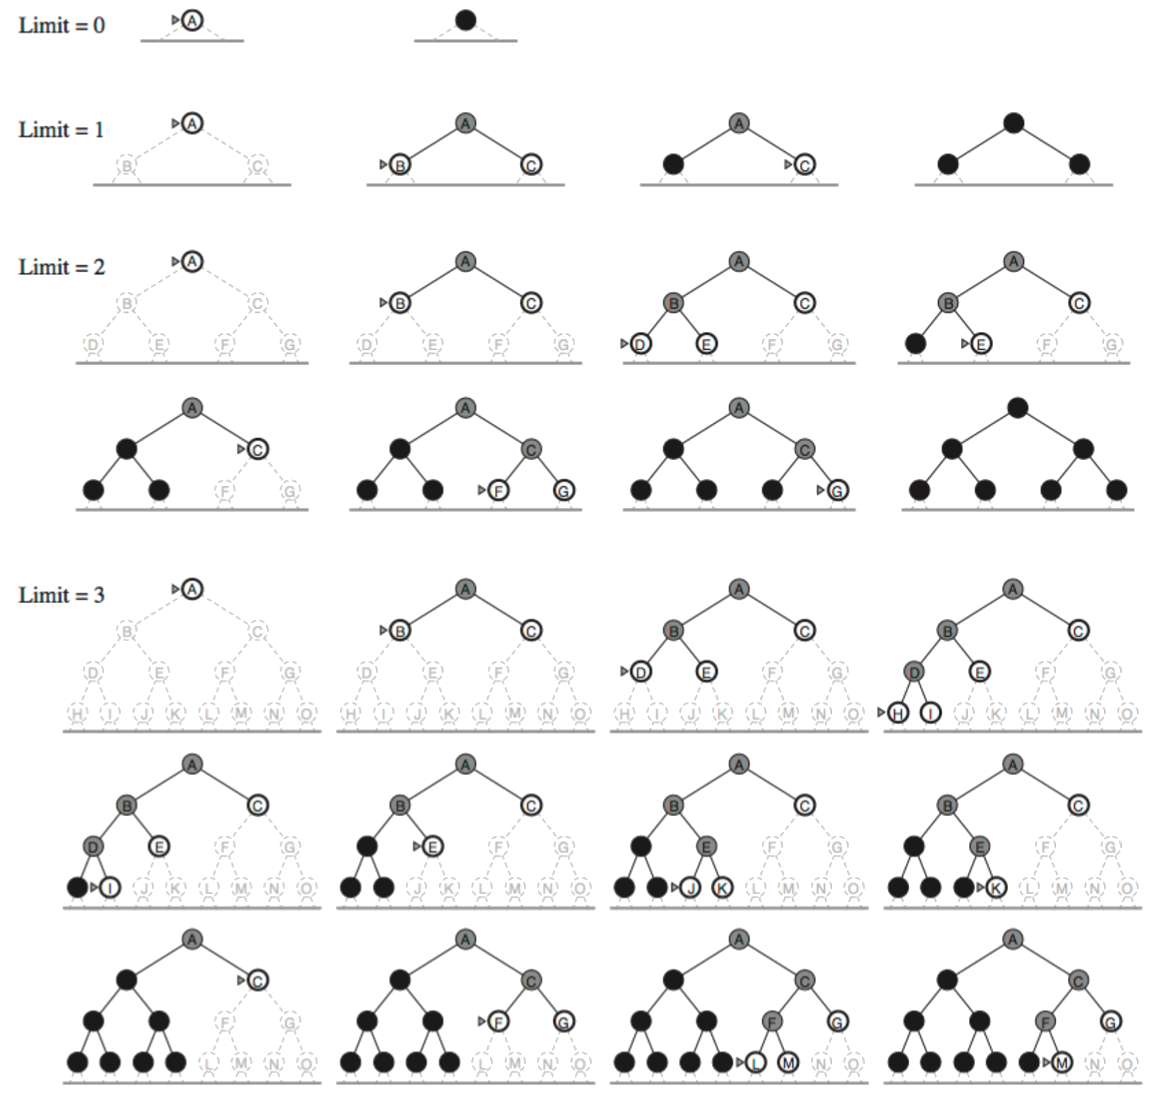
\includegraphics[width=.6\linewidth]{./figures/iddfs.png}
\end{center}


\end{frame}

\begin{frame}[c]{STRIPS + IDDFS + Prolog = Exercise}
    
    \startExercise

    \begin{block}{Exercise \currentExercise}
        Edit the \prolog{strips/3} and \prolog{strips_impl/6} rules in \texttt{Strips.pl} in such a way that your STRIPS implementation performs an IDDFS for plans, up to \prolog{max_depth(MD)}
        %
        \begin{itemize}
            \item assume \prolog{max_depth(MD)} is part of your theory
            %
            \begin{itemize}
                \item the value of \prolog{MD} actually coincides with the value of the \texttt{maxDepth} entry in \texttt{gradle.properties}
            \end{itemize}

            \item test it against the \texttt{Registers.pl} world

            \item notice that the \prolog{BadActions} tricks should became useless
        \end{itemize}
    \end{block}


\end{frame}

%===============================================================================
\section*{}
%===============================================================================

%/////////
\frame{\titlepage}
%/////////

%===============================================================================
\section*{\refname}
%===============================================================================

% %%%%
% \setbeamertemplate{page number in head/foot}{}
% %/////////
% \begin{frame}[c,noframenumbering]{\refname}
% %\begin{frame}[t,allowframebreaks,noframenumbering]{\refname}
% %	\tiny
% 	\scriptsize
% %	\footnotesize
% 	\nocite{*}
% 	\bibliographystyle{apalike-AMS}
% 	\bibliography{ise-lab-strips}
% \end{frame}
% % /////////

%%%%%%%%%%%%%%%%%%%%%%%%%%%%%%%%%%%%%%%%%%%%%%%%%%%%%%%%%%%%%%%%%%%%%%%%%%%%%%%%
\end{document}
%%%%%%%%%%%%%%%%%%%%%%%%%%%%%%%%%%%%%%%%%%%%%%%%%%%%%%%%%%%%%%%%%%%%%%%%%%%%%%%%
